%%%%%%%%%%%%%%%%%%%%%%%%%%%%%%%%%%%%%%%%%%%%%%%%%%%%%%%%%%%%%%%%%%%%%%%%%%
%%%%%%%%%%%%%%%%%%%%%%%%%%%%%%%%%%%%%%%%%%%%%%%%%%%%%%%%%%%%%%%%%%%%%%%%%%%
%%% Inference rules for binary predicates
%%% Stephen J. Hegner
%%% Section 5
%%% 29 July 2021
%%%%%%%%%%%%%%%%%%%%%%%%%%%%%%%%%%%%%%%%%%%%%%%%%%%%%%%%%%%%%%%%%%%%%%%%%%%
%%%%%%%%%%%%%%%%%%%%%%%%%%%%%%%%%%%%%%%%%%%%%%%%%%%%%%%%%%%%%%%%%%%%%%%%%%%



 \section{Inference for Positive Binary Granular Constraints}\label{sec:pinfrules}

    In this section, a complete inference system is developed for
 $\pbinconstrgrsch{G}$; \ie, for binary rules of the form
\mbox{$\subrulep{g_1}{g_2}$} and \mbox{$\disjrulep{g_1}{g_2}$}.  It is
based substantially upon \mycite{AtzeniPa88_dke}, although significant
differences in the two frameworks (particularly, the absence of the
granules $\botgrsch{G}$ and $\topgrsch{G}$ in
\mycite{AtzeniPa88_dke}), as well as the need to ensure that proofs
are single use (a property not considered in \mycite{AtzeniPa88_dke}),
render the task substantial.
     \par
    While the presentation here is designed to be independent of
\mycite{AtzeniPa88_dke}, referring to the latter only for proofs,
readers may nevertheless be interested in consulting that work as a
reference point.  To that end, a brief summary of the terminology and
notation of \mycite{AtzeniPa88_dke}\footnote{
    \mycite{AtzeniPa86_icde} is a preliminary conference version of
the journal article \mycite{AtzeniPa88_dke}.  Readers who have
difficulty accessing \mycite{AtzeniPa88_dke} may find
\mycite{AtzeniPa86_icde} a useful alternative.}
 is provided below.


 \begin{metalabpara}{summary}{}
         {Summary of terminology, notation, and context of 
                \protect\mycite{AtzeniPa88_dke}}\envlabel{sum:AP}
    The work of \mycite{AtzeniPa88_dke} has its roots in general
knowledge bases, and so uses different terminology and notation than
does this report, whose roots are in the spatial domain.
     In \mycite{AtzeniPa88_dke}, the equivalent of an SMAS is called a
\emph{scheme}, with \emph{types} corresponding to the granules of an
SMAS, and \emph{objects} corresponding to the elements of the domain
$\gnledom{\sigma}$ of a granule structure $\sigma$.  A \emph{potential
state} assigns objects to types, much as the function
$\gnletodom{\sigma}$ assigns domain elements to granules.
    The subsumption constraint $\subrulep{g_1}{g_2}$ of this paper is
written $\isa{g_1}{g_2}$, while the disjointness constraint
$\disjrulep{g_1}{g_2}$ is written $\disj{g_1}{g_2}$.
     \par
    From the perspective of semantics, there are two significant
points of difference with the SMAS framework of this paper.  First,
there are no specially identified types corresponding to
$\botgrsch{G}$ and $\topgrsch{G}$, although it is possible to require
that a type $g$ be assigned the empty set of objects via the
constraint $\disj{g}{g}$.  Such a type is termed \emph{inconsistent},
with a scheme \emph{inconsistent} if it contains at least one
inconsistent type.  Second, the set of objects associated with a type
is not required to be nonempty.  This is in sharp contrast to the SMAS
framework, in which a granule structure assigns to each granule, other
than $\botgrsch{G}$, a \emph{nonempty} set of domain elements.
 \end{metalabpara}

 
 \begin{metalabpara}{mydefinition}{}
  {Granule quasi-structures and quasi-models}\envlabel{def:quasi}
     In \mycite{AtzeniPa88_dke}, a more relaxed version of (the notion
corresponding to) a granule structure $\sigma$ than employed in an
SMAS (see \envref{def:granstrsem}) is used, in which there are no
restrictions on the mapping $\gnletodom{\sigma}$.
     To keep the distinction clear, a structure in the sense of
\mycite{AtzeniPa88_dke} will be termed a quasi-structure.
     Formally, a \emph{granule quasi-structure} over
$\granschemaname{G}$ is a pair $\gnlestrpr{\sigma}$ in which
$\gnledom{\sigma}$ is a nonempty set and
  $\fn{\gnletodom{\sigma}}{\granulesofsch{G}}
                          {\powerset{\gnledom{\sigma}}}$
 is a function which assigns a subset of $\gnledom{\sigma}$ to each
granule, subject to the further property that
   $\bigunion\setdef{\gnletodom{\sigma}(g)}{g \in \granulesofsch{G}}
                        = \gnledom{\sigma}$.
     Note in particular that there is no requirement that granules
other than $\botgrsch{G}$ map to nonempty sets, and there are no
restrictions on the images of $\botgrsch{G}$ or $\topgrsch{G}$.
     There is, however, the weaker property that every domain element
occur in the image of some granule under $\gnletodom{\sigma}$.
     \par
   A granule quasi-structure $\sigma$ is a \emph{quasi-model} of the
subsumption constraint $\subrulep{g_1}{g_2}$ if
 $\gnletodom{\sigma}(g_1) \subseteq \gnletodom{\sigma}(g_2)$, and it
is a quasi-model of the disjointness constraint $\disjrulep{g_1}{g_2}$
if 
 $\gnletodom{\sigma}(g_1) \intersect \gnletodom{\sigma}(g_2)
                                    = \emptyset$.
   For $\Phi \subseteq \pbinconstrgrsch{G}$, $\sigma$ is a quasi-model
of $\Phi$ if it is a quasi-model of each $\varphi \in \Phi$.
   Finally, it is a quasi-model for $\granschemaname{G}$ if it is a
quasi-model of $\constrgrsch{G}$ (but not necessarily of
$\pbintautgrsch{G}$).
     \par
   The \emph{empty quasi-structure} over $\granschemaname{G}$, denoted
$\emptyqs{G}$, has $\gnledom{\emptyqs{G}} = \emptyset$ with
 $\gnletodom{\emptyqs{G}}$ the function which maps every granule to
$\emptyset$.  This quasi-structure is interesting primarily because it
is always a quasi-model, thus showing that any SMAS is satisfiable in
the context of quasi-models.
     \par
     To avoid confusion with quasi-models, the granule structures
(resp.\  models) of this
paper will sometimes be called \emph{full structures}
(resp.\ \emph{full models}).
 \end{metalabpara}


\begin{metalabpara}{summary}{}
  {Inference rules on quasi-models}\envlabel{sum:APinf}
    The inference rules of \mycite[Lem.\ 3]{AtzeniPa88_dke} are shown
in Fig.\ \ref{fig:qbininfpos}.
    Define the inference system $\qbininfpos{G}$ to have
  \nlrightt
  $\infrulesof{\qbininfpos{G}} = 
     \setbr{\text{(I1)}, \text{(I2)}, \text{(D1)},
            \text{(M1)}, \text{(M2)} }$.
   \newline
   \begin{figure}[htb]
   \def\isepi{0.5em}
   \begin{align*}
   &\mbox{(I2)}\hspace*{\isepi}
    \begin{prooftreem}
       \hypoii{\subrulep{\granvar{g}_1}{\granvar{g}_2}}
              {\subrulep{\granvar{g}_2}{\granvar{g}_3}}
       \inferi{\subrulep{\granvar{g}_1}{\granvar{g}_3}}
    \end{prooftreem}
   &&\mbox{(M1)}\hspace*{\isepi}
    \begin{prooftreem}
      \hypoii{\subrulep{\granvar{g}_1}{\granvar{g}_1'}}
              {\disjrulep{\granvar{g}_1'}{\granvar{g}_2}}
      \inferi{\disjrulep{\granvar{g}_1}{\granvar{g}_2}}
    \end{prooftreem}
    \end{align*}
    \begin{align*}
   &\mbox{(I1)}\hspace*{\isepi}
    \begin{prooftreem}
      \hypoi{\phantom{X}}
      \inferi{\subrulep{\granvar{g}}{\granvar{g}}}
    \end{prooftreem}
   &&\mbox{(D1)}\hspace*{\isepi}
    \begin{prooftreem}
      \hypoi{\disjrulep{\granvar{g}'}{\granvar{g}'}}
      \inferi{\disjrulep{\granvar{g}'}{\granvar{g}}}
    \end{prooftreem}
   &&&\mbox{(M2)}\hspace*{\isepi}
    \begin{prooftreem}
      \hypoi{\disjrulep{\granvar{g}'}{\granvar{g}'}}
      \inferi{\subrulep{\granvar{g'}}{\granvar{g}}}
    \end{prooftreem}
   \end{align*}
   \caption{Inference rules of $\qbininfpos{G}$}\label{fig:qbininfpos}
   \end{figure}
     The main rules are (I2) and (M1), which assert that subsumption
is transitive, and that disjointness is preserved under reduction of
granule size via subsumption, respectively.
     The rule (I1) asserts the tautology that every granule subsumes
itself.  These three rules make sense equally in the contexts of full
models and quasi-models.
     \par
     The remaining two rules, (D1) and (M2), assert that if a granule
is disjoint from itself, then it is also disjoint from every other
granule as well, and is also subsumed by every granule, respectively.
This makes sense in the context of quasi-models, since any granule in
a quasi-model may be required to be empty.  However, in the context of
full models, they rules apply only to the case that $\granvar{g}'$ is
bound to $\botgrsch{G}$.  This is explained in more detail in
\envref{def:bininfpos} and \envref{prop:bininfpos}.
 \end{metalabpara}


 \begin{metaemphlabpara}{proposition}{Proposition}
   {Soundness and completeness of $\qbininfpos{G}$}\envlabel{prop:qbininfpos}
   The inference rules of $\qbininfpos{G}$, shown in
Fig.\ \ref{fig:qbininfpos} are sound and complete in the context of
quasi-models.
    More precisely, they are complete when the concept of model used
is that of quasi-model.
 \begin{proof}
  See \mycite[Thm.\ 1]{AtzeniPa88_dke}.
 \end{proof}
 \end{metaemphlabpara}
    \parvert

   The strategy of augmenting $\qbininfpos{G}$ to obtain an inference
system which is complete for full models is a straightforward, and is
executed in two steps.  In the first, additional rules which enforce
all members of $\pbintautgrsch{G}$ as constraints are added, and in
the second, additional rules which require that the members of
$\pbinunsatgrsch{G}$ can never be satisfied are added.  The details
follow.


 \begin{metalabpara}{mydefinition}{}
  {Strong quasi-structures and quasi-models}\envlabel{def:squasistr}
     Call quasi-structure $\gnlestrprii{\sigma}$ over
$\granschemaname{G}$ \emph{strong} if
$\gnletodom{\sigma}(\botgrsch{G}) = \emptyset$ and
 $\gnletodom{\sigma}(\topgrsch{G}) = \gnledom{\sigma}$.
    A quasi-model of $\granschemaname{G}$ which is also a strong
quasi-structure is called a \emph{strong quasi-model} (of
$\granschemaname{G}$).
    \par
    Clearly, every full structure (resp.\ full model) is also a strong
quasi-structure (resp.\ strong quasi-model).  The only difference is
that in a strong quasi-structure $\sigma$, there is no requirement
that $\gnletodom{\sigma}(g) \neq \emptyset$ for $g \in
\granulesofschnb{G}$.
    \par
    Also, note that $\emptyqs{G}$ is always a strong quasi-model,
whatever be $\constrgrsch{G}$.  Thus, just as is the case for ordinary
quasi-structures, any SMAS is satisfiable in the context of strong
quasi-models.
 \end{metalabpara}


 \begin{metaemphlabpara}{proposition}{Proposition}
   {Tautologies and strong quasi-structures}\envlabel{prop:strongqstr}
    If $\sigma$ is a quasi-
 \preformat{\linebreak}
 structure over $\granschemaname{G}$ which
furthermore satisfies $\pbintautgrsch{G}$, then it is a strong
quasi-structure over $\granschemaname{G}$.
    Consequently, if $\sigma$ is a quasi-model of $\granschemaname{G}$
which satisfies $\pbintautgrsch{G}$, then it is a strong quasi-model.
 \begin{proof}
    The two differences between $\gnlestrpr{\sigma}$ being an ordinary
quasi-structure and a strong quasi-structure are that, in the latter,
it is additionally required that
 \preformat{\linebreak}
    (a) $\gnletodom{\sigma}(\botgrsch{G})=\emptyset$; and
    (b) $\gnletodom{\sigma}(\topgrsch{G})=\gnledom{\sigma}$.
  In a quasi-structure, neither of these conditions is required to hold.
  To prove the assertion, it suffices to show that requiring that all
constraints in $\pbintautgrsch{G}$ hold implies that (a) and (b) hold.
This is easily verified, as follows.
     \par
   For (a), letting $g \ideq \botgrsch{G}$ in
 $\disjrulep{\botgrsch{G}}{g} \in \pbintautgrsch{G}$,
 it follows that
 \preformat{\linebreak}
 $\gnletodom{\sigma}(\botgrsch{G})
     \intersect \gnletodom{\sigma}(\botgrsch{G}) = \emptyset$,
 which can only hold if
 $\gnletodom{\sigma}(\botgrsch{G}) = \emptyset$.
     \par
   For (b), the tautology
  $\subrulep{g}{\topgrsch{G}} \in \pbintautgrsch{G}$ guarantees that
 $\gnletodom{\sigma}(g) \subseteq \gnletodom{\sigma}(\topgrsch{G})$
 for every $g \in \granulesofsch{G}$, which with the additional
condition
 \preformat{\linebreak}
   $\bigunion\setdef{\gnletodom{\sigma}(g)}{g \in \granulesofsch{G}}
                        = \gnledom{\sigma}$
  (see \envref{def:quasi})
 guarantees that
     $\gnletodom{\sigma}(\topgrsch{G}) = \gnledom{\sigma}$,
 completing the proof.
 \end{proof}
 \end{metaemphlabpara}


 \begin{metalabpara}{mydefinition}{}
  {Extending $\qbininfpos{G}$
           to strong quasi-models}\envlabel{def:sqbininfpos}
    Define the inference system
 \preformat{\linebreak}
 $\sqbininfpos{G}$ to have
  \nlrightt
  $\infrulesof{\sqbininfpos{G}} =
        \infrulesof{\qbininfpos{G}} \union
     \setbr{\text{(T1)}, \text{(T2)}, \text{(T3)}}$,
   \newline
  with the rules (T1), (T2), and (T3) as defined in
Fig.\ \ref{fig:tautbininfpos}.
   \begin{figure}[htb]
   \def\isepi{0.5em}
   \begin{align*}
   &\mbox{(T1)}\hspace*{\isepi}
    \begin{prooftreem}
      \hypoi{\phantom{X}}
      \inferi{\disjrulep{\botgrsch{G}}{\granvar{g}}}
    \end{prooftreem} 
   &&\mbox{(T2)}\hspace*{\isepi}
    \begin{prooftreem}
      \hypoi{\phantom{X}}
      \inferi{\subrulep{\botgrsch{G}}{\granvar{g}}}
    \end{prooftreem}
   &&&\mbox{(T3)}\hspace*{\isepi}
    \begin{prooftreem}
      \hypoi{\phantom{X}}
      \inferi{\subrulep{\granvar{g}}{\topgrsch{G}}}
    \end{prooftreem}
    \end{align*}
   \caption{Additional tautological rules $\sqbininfpos{G}$}\label{fig:tautbininfpos}
   \end{figure}
 \end{metalabpara}


 \begin{metaemphlabpara}{proposition}{Proposition}
   {Soundness and completeness of $\sqbininfpos{G}$
     in the context of strong quasi-models}\envlabel{prop:sqbininfpos}
   The inference rules of $\sqbininfpos{G}$ are sound and complete in
the context of strong quasi-models.
    More precisely, they are complete when the concept of model used
is that of strong quasi-model.
 \begin{proof}
    The result follows from \envref{prop:strongqstr}, together with
the fact that the added rules (T1), (T2), and (T3) of
$\sqbininfpos{G}$, together with (I1) of $\qbininfpos{G}$, force all
constraints in $\pbintautgrsch{G}$ to hold.
 \end{proof}
 \end{metaemphlabpara}


 \begin{metaemphlabpara}{proposition}{Proposition}
   {Strong quasi-structures
        and $\pbinunsatgrsch{G}$}\envlabel{prop:strongqstrunsat}
    If $\sigma$ is a strong quasi-structure over $\granschemaname{G}$
which has the further property that for no
 $\varphi \in \pbinunsatgrsch{G}$
 is it the case that
 $\constrgrsch{G} \union \pbintautgrsch{G} \sentails \varphi$,
 then $\sigma$ is a (full) structure over $\granschemaname{G}$.
    \par
    Consequently, if $\sigma$ is a strong quasi-model of
$\granschemaname{G}$ which does not satisfy any member of
$\pbinunsatgrsch{G}$, then it is a (full) model of
$\granschemaname{G}$.
 \begin{proof}
    The difference between $\gnlestrpr{\sigma}$ being a strong
quasi-structure and a full structure is that, in the latter, it is
additionally required that, for $g \in \granulesofschnb{G}$,
         $\gnletodom{\sigma}(g)\neq\emptyset$.
   Now, for any $g \in \granulesofschnb{G}$, it is the case that
   $\disjrulep{g}{g} \in \pbinunsatgrsch{G}$,
 which forbids
   $\gnletodom{\sigma}(g)
       =\gnletodom{\sigma}(g) \intersect \gnletodom{\sigma}(g)
          = \emptyset$.
 \end{proof}
 \end{metaemphlabpara}


 \begin{metaemphlabpara}{theorem}{Theorem}
   {Sat-completeness of $\sqbininfpos{G}$}\envlabel{thm:satcomplsbin}
   The inference rules of
  \preformat{\linebreak}
 $\sqbininfpos{G}$ are sound and sat-complete in the context of full
models.
 \begin{proof}
    The result follows from \envref{prop:sqbininfpos} and
\envref{prop:strongqstrunsat}, since for sat-completeness, the
possibility of a structure satisfying any member of
$\pbinunsatgrsch{G}$ is ruled out.
 \end{proof}
 \end{metaemphlabpara}


 \begin{metalabpara}{mydefinition}{}
  {Extending $\sqbininfpos{G}$ to models}\envlabel{def:qbininfposext}
    Define the inference system
 \preformat{\linebreak}
 $\sqbininfposext{G}$ to have
  \nlrightt
  $\infrulesof{\sqbininfposext{G}} =
        \infrulesof{\sqbininfpos{G}} \union
            \setbr{\text{(U1)}, \text{(U2)} }$,
   \newline
  with the rules (U1) and (U2) as defined in
Fig.\ \ref{fig:sqbininfposadd}.
   \begin{figure}[htb]
   \def\isepi{0.5em}
   \begin{align*}
    &\mbox{(U1)}\hspace*{\isepi}
    \begin{prooftreem}
      \hypoi{\disjrulep{\granvar{g}}{\granvar{g}}}
      \inferi{\false}
    \end{prooftreem}
    {\scriptstyle\abr{|{\scriptscriptstyle(\granvar{g} \neq \botgrsch{G})}}}
   &&\mbox{(U2)}\hspace*{\isepi}
    \begin{prooftreem}
      \hypoi{\subrulep{g}{\botgrsch{G}}}
      \inferi{\false}
    \end{prooftreem}
    {\scriptstyle\abr{|{\scriptscriptstyle(\granvar{g} \neq \botgrsch{G})}}}
    \end{align*}
   \caption{Additional rules of $\sqbininfposext{G}$}\label{fig:sqbininfposadd}
   \end{figure}
 \end{metalabpara}


 \begin{metaemphlabpara}{proposition}{Proposition}
   {Soundness and completeness of $\qbininfposext{G}$
     in the context of full models}\envlabel{prop:qbininfposext}
   The inference rules of $\sqbininfposext{G}$ are sound and complete in
the context of full models.
 \begin{proof}
   Soundness and sat-completeness follow from
\envref{thm:satcomplsbin}, while (U1) and (U2) ensure that
unsatisfiability will be detected.
 \end{proof}
 \end{metaemphlabpara}


 \begin{metalabpara}{mydefinition}{}
  {Unnecessary rules of $\bininfpossat{G}$}\envlabel{def:bininfpos}
    While the inference system
 \preformat{\linebreak}
 $\qbininfposext{G}$ is sound and complete for full models, it
contains some rules which are not necessary.  Specifically, the rules
(D1), (M2), and (U2) may be removed.  Define the inference system
$\bininfpos{G}$ to have
  \nlrightt
  $\infrulesof{\bininfpos{G}}
      = (\infrulesof{\sqbininfposext{G}}
              \setminus \setbr{\text{(D1)},\text{(M2)},\text{(U2)}}$.
   \newline
   Due to its importance, this inference system is shown in full in
Fig.\ \ref{fig:bininfpos}.
   \begin{figure}[htb]
   \def\isepi{0.5em}
   \begin{align*}
   &\mbox{(I2)}\hspace*{\isepi}
    \begin{prooftreem}
       \hypoii{\subrulep{\granvar{g}_1}{\granvar{g}_2}}
              {\subrulep{\granvar{g}_2}{\granvar{g}_3}}
       \inferi{\subrulep{\granvar{g}_1}{\granvar{g}_3}}
    \end{prooftreem}
   &&\mbox{(M1)}\hspace*{\isepi}
    \begin{prooftreem}
      \hypoii{\subrulep{\granvar{g}_1}{\granvar{g}_1'}}
              {\disjrulep{\granvar{g}_1'}{\granvar{g}_2}}
      \inferi{\disjrulep{\granvar{g}_1}{\granvar{g}_2}}
    \end{prooftreem}
    \end{align*}
    \begin{align*}
   &\mbox{(I1)}\hspace*{\isepi}
    \begin{prooftreem}
      \hypoi{\phantom{X}}
      \inferi{\subrulep{\granvar{g}}{\granvar{g}}}
    \end{prooftreem}
   &&\mbox{(T1)}\hspace*{\isepi}
    \begin{prooftreem}
      \hypoi{\phantom{X}}
      \inferi{\disjrulep{\botgrsch{G}}{\granvar{g}}}
    \end{prooftreem} 
   &&&\mbox{(T2)}\hspace*{\isepi}
    \begin{prooftreem}
      \hypoi{\phantom{X}}
      \inferi{\subrulep{\botgrsch{G}}{\granvar{g}}}
    \end{prooftreem}
   &&&&\mbox{(T3)}\hspace*{\isepi}
    \begin{prooftreem}
      \hypoi{\phantom{X}}
      \inferi{\subrulep{\granvar{g}}{\topgrsch{G}}}
    \end{prooftreem}
    \end{align*}
    \begin{align*}
    &\mbox{(U1)}\hspace*{\isepi}
    \begin{prooftreem}
      \hypoi{\disjrulep{\granvar{g}}{\granvar{g}}}
      \inferi{\false}
    \end{prooftreem}
    {\scriptstyle\abr{|{\scriptscriptstyle(\granvar{g} \neq \botgrsch{G})}}}
   \end{align*}
   \caption{Inference rules of $\bininfpos{G}$}\label{fig:bininfpos}
   \end{figure}
    That it is sound and complete for full model is established in
\envref{prop:bininfpos} below.
 \end{metalabpara}


 \begin{metaemphlabpara}{proposition}{Proposition}
   {Soundness and completeness of $\bininfpos{G}$}\envlabel{prop:bininfpos}
   The inference rules of $\bininfpos{G}$ are sound and complete in
the context of full models.
 \begin{proof}
   First of all, the premise $\disjrulep{\granvar{g}'}{\granvar{g}'}$
in rules (D1) and (M2) can only hold in the case that $\granvar{g}'$
is bound to $\botgrsch{G}$, in view of rule (U1).  Since
$\disjrulep{\botgrsch{G}}{\botgrsch{G}}$ is a tautology by (T1), the
premise for $\granvar{g}$ bound to $\botgrsch{G}$ becomes $\true$ in
both (D1) and (M2).  The resulting rules are precisely (T1) and (T2),
respectively, rendering the original (D1) and (M2) unnecessary.
    \par
   To justify removing (U2), it suffices that to note that the
unsatisfiability of $\subrulep{g}{\botgrsch{G}}$ may be deduced from
the unsatisfiability of $\disjrulep{g}{g}$, using additionally (T2)
and (M1), as shown in Fig.\ \ref{fig:dedunsat}.
   \begin{figure}[htb]
   \[
     \begin{prooftreem}
      \hypoi{\subrulep{\granvar{g}}{\botgrsch{G}}}
      \hypoi{\phantom{X}}
      \inferi{\disjrulep{\botgrsch{G}}{\granvar{g}}}
      \inferii{\disjrulep{\granvar{q}}{\granvar{q}}}
      \inferi{\false}
     \end{prooftreem}
    {\scriptstyle\abr{|{\scriptscriptstyle(\granvar{g} \neq \botgrsch{G})}}}
   \]
   \caption{Deducing the unsatisfiability of
                $\subrulep{\granvar{g}}{\botgrsch{G}}$
           from that of 
                $\disjrulep{\granvar{g}}{\granvar{g}}$}\label{fig:dedunsat}
   \end{figure}
 \end{proof}
 \end{metaemphlabpara}


 \begin{metalabpara}{discussion}{}
   {Armstrong context strategy}\envlabel{disc:barmstrong}
     The approach to extending inference systems such as
$\bininfpos{G}$ to include negative constraints as well requires that
the context (in this case $\pbinconstrgrsch{G}$) be Armstrong (see
\envref{summ:armstrong}).
     A straightforward way to show that a context is Armstrong is to
use the characterization given in \mycite[Thm.\ 3.1]{Fagin82}.  The
proof has already been developed in
\mycite[3.15-3.18]{HegnerRo17_inform} for a much more general class of
granular constraints than $\pbinconstrgrsch{G}$, and so will not be
repeated here.  The reader is referred to that article for details.
For completeness, the formal result is recorded below.
 \end{metalabpara}


 \begin{metaemphlabpara}{theorem}{Theorem}
   {Armstrong context}\envlabel{thm:barmstrong}
     $\pbinconstrgrsch{G}$ is an Armstrong context.
 More precisely, if $\granschemaname{G}$ is satisfiable, then
 $\pconstrgrsch{G} \union \pbintautgrsch{G}$ admits an Armstrong
model.
 \begin{proof}
    See \mycite[3.18]{HegnerRo17_inform}.
 \end{proof}
 \end{metaemphlabpara}
    \parvert

   Attention is now turned to the task of showing that proofs in
$\bininfpos{G}$ are single use.  For this task, it is useful to begin
by characterizing properties of $\granschemaname{G}$ via an associated
graph.

 \begin{metalabpara}{mydefinition}{}
         {The graph of an SMAS}\envlabel{def:graphsmas}
     The \emph{graph} of $\granschemaname{G}$, denoted
$\graphofgrsch{G}$, has as vertices the elements of
$\granulesofsch{G}$.  It has two types of edges, one directed and one
undirected, defined as follows.
    \baxblkc
      \axitem{(s-edge)} For $g_1, g_2 \in \granulesofsch{G}$, there is
a directed \emph{subsumption edge} from $g_1$ to $g_2$ just in case
     $\subrulep{g_1}{g_2} \in
          \pconstrgrsch{G} \union \pbintautgrsch{G}$.
   Formally, this edge is regarded as the ordered pair
$\grpr{g_1}{g_2}$.
   The set of all subsumption edges of $\graphofgrsch{G}$ is denoted
$\sedgesofgrsch{G}$.
      \axitem{(d-edge)} For $g_1, g_2 \in \granulesofsch{G}$, there is
an undirected \emph{disjointness edge} between $g_1$ and $g_2$ just in
case
     $\disjrulep{g_1}{g_2} \in \pconstrgrsch{G} \union
\pbintautgrsch{G}$.
   Formally, if $g_1 \not\ideq g_2$, this edge is regarded as the
unordered pair $\setbr{g_1,g_2}$.  In the case that $g_1 \ideq g_2$, 
it is regarded as the singleton
  $\setbr{g_1} = \setbr{g_2} = \setbr{g_1,g_2}$.
   The set of all disjointness edges of $\graphofgrsch{G}$ is denoted
$\dedgesofgrsch{G}$.
    \eaxblk
   The set of \emph{all edges} of $\graphofgrsch{G}$ is
  \nlrightt
   $\edgesofgrsch{G} = \sedgesofgrsch{G} \union \dedgesofgrsch{G}$.
  \newline
   In the equivalent of this graph in \mycite{AtzeniPa88_dke},
subsumption edges are called \emph{black edges} and disjointness edges
are called \emph{red edges}.
     \par
    A \emph{subsumption path} in $\graphofgrsch{G}$ is a sequence
 $p = \abr{g_1,g_2,\ldots,g_k}$, with $k \geq 2$,
 of elements of $\granulesofsch{G}$ with the property that for
each $i \in \ccinterval{1}{k-1}$,
 $\grpr{g_i}{g_{i+1}} \in \sedgesofgrsch{G}$.
   Such a path $p$ is said to be \emph{from} $g_1$ \emph{to} $g_k$,
and to \emph{underlie} $\grpr{g_1}{g_k}$.
   The set of all subsumption paths of $\graphofgrsch{G}$ is denoted
$\spathsofgrsch{G}$.
   The length $k$ of $p$ is denoted $\lengthof{p}$.
    \par
    The \emph{underlying constraint sequence} of $p$ is
 $\constrseq{p} =
   \abr{\subrulep{g_1'}{g_2'},\subrulep{g_2'}{g_3'},\ldots,
      \subrulep{g_i'}{g_{i+1}'},\ldots,\subrulep{g_{k-1}'}{g_k'}}$,
 with $\subrulep{g_i'}{g_{i+1}'}$ the \emph{$i^{th}$-constraint} of
$p$.
   The \emph{underlying constraint set} of $p$ is the underlying
constraint sequence with the order removed; more precisely,
 $\constrset{p} =
   \setbr{\subrulep{g_1'}{g_2'},\subrulep{g_2'}{g_3'},\ldots,
      \subrulep{g_i'}{g_{i+1}'},\ldots,\subrulep{g_{k-1}'}{g_k'}}$,
    \par
   The relation $\sstaredgesofgrsch{G}$ on $\granulesofsch{G}$ is
defined by
  $\grpr{g_1}{g_2} \in
 \preformat{\linebreak}
 \sstaredgesofgrsch{G}$
 iff there is a
 $\abr{g_1',g_2',\ldots,g_k'} \in \spathsofgrsch{G}$
 with $g_1' \ideq g_1$ and $g_k' \ideq g_2$.
  In this case, the path $p = \abr{g_1',g_2',\ldots,g_k'}$ is said to
\emph{underlie} $\grpr{g_1}{g_2}$.
 \end{metalabpara}


 \begin{metaemphlabpara}{proposition}{Proposition}
    {Existence of underlying paths}\envlabel{prop:underpaths}
    Let $g_1, g_2 \in \granulesofsch{G}$, and assume further that 
$\granschemaname{G}$ is satisfiable.
    Then the entailment
        $\pconstrgrsch{G} \union \pbintautgrsch{G}
                      \sentails \subrulep{g_1}{g_2}$
   holds iff there is a subsumption path $p$ which underlies
$\grpr{g_1}{g_2}$.
 \begin{proof}
  That the result then holds in the context of quasi-models is shown
in \mycite[Thm.\ 2]{AtzeniPa88_dke}.  Upon adding the tautologies and
taking into account the results of \envref{prop:strongqstr}, it is
easy to see that it holds in the context of strong quasi-models as
well.
    Finally, with the requirement that $\granschemaname{G}$ be
satisfiable, in view of \envref{prop:strongqstrunsat}, the result
applies to the context of full models also.
 \end{proof}
 \end{metaemphlabpara}
    \parvert

    Since a subsumption constraint holds in $\granschemaname{G}$ iff
it has an underlying path, it also has a simple proof based upon that
path.  The details follow.

 \begin{metalabpara}{}{}
    {Linear proofs for subsumption constraints}\envlabel{def:linearproof}
     Let $p' = \abr{g_1',g_2',\ldots,g_k'} \in
 \preformat{\linebreak}
 \spathsofgrsch{G}$.
     The \emph{left-linear proof tree} (in $\bininfpos{G}$) associated
with $p$, denoted
 $\llinear{p}$, is defined as follows.
  \baxblkc
   \axitem{(a)} If $k=2$ and
 $\subrulep{g_1'}{g_2'} \in \constrgrsch{G}$, then $\llinear{p}$ is
simply $\subrulep{g_1'}{g_2'}$.
   In this case, the proof uses no rules at all, since the desired
consequence is in the set of antecedents.
   \axitem{(b)} If $k=2$ and
 $\subrulep{g_1'}{g_2'} \in \pbintautgrsch{G}\setminus\constrgrsch{G}$,
 then $\llinear{p}$ is the tree $\subrulepbar{g_1'}{g_2'}{0}$.
     In this case, the proof uses at most the rules in
 $\setbr{\text{(I1)},\text{(T1)},\text{(T2)},\text{(T3)}}$.
   \axitem{(c)} If $k>2$ and for every $i \in \ccinterval{1}{k-1}$ it
is the
 case that $\subrulep{g_i'}{g_{i+1}'} \in \constrgrsch{G}$, then
$\llinear{p}$ is defined as shown in Fig.\ \ref{fig:llinearp} .
   \begin{figure}[htb]
   \[
     \begin{prooftreem}
      \hypoii{\subrulep{g_1'}{g_2'}}
             {\subrulep{g_2'}{g_3'}}
      \inferi{\subrulep{g_1'}{g_3'}}
      \hypoi{\subrulep{g_3'}{g_4'}}
      \inferii{\subrulep{g_1'}{g_4'}}
      \ellipsis{}{\subrulep{g_1'}{g_{i}'}}
      \hypoi{\subrulep{g_i'}{g_{i+1}'}}
      \inferii{\subrulep{g_1'}{g_{i+1}'}}
      \ellipsis{}{\subrulep{g_1'}{g_{k-1}'}}
      \hypoi{\subrulep{g_k'}{g_{k-1}'}}
      \inferii{\subrulep{g_{1}'}{g_{k}'}}
     \end{prooftreem}
   \]
   \caption{A left-linear proof tree for subsumption}\label{fig:llinearp}
   \end{figure}
   In this case, only rule (I2) is used.
   \axitem{(d)} If $k>2$ and for one or more
 $i \in \ccinterval{1}{k-1}$ it is the case that
 $\subrulep{g_i'}{g_{i+1}'}
                     \in \pbintautgrsch{G}\setminus\constrgrsch{G}$,
 then
 $\llinear{p}$ is as shown in Fig.\ \ref{fig:llinearp}, but with
  $\subrulep{g_i'}{g_{i+1}'}$ replaced by the tree
$\subrulepbar{g_i'}{g_{i+1}'}{1.5}$.
  In this case, at most the rules in 
 $\setbr{\text{(I1)},\text{(I1)},\text{(T1)},\text{(T2)},\text{(T3)}}$
 are used.
  \eaxblk     
 \end{metalabpara}


 \begin{metaemphlabpara}{lemma}{Lemma}
    {Existence of left-linear proofs}\envlabel{lem:llinear}
    Let $g_1, g_2 \in \granulesofsch{G}$.  If $\granschemaname{G}$ is
satisfiable and
 $\pbinconstrgrsch{G} \union \pbintautgrsch{G}
         \sentails \subrulep{g_1}{g_2}$,
 then there is a left-linear proof of this in $\bininfpos{G}$.
 \begin{proof}
   Use \envref{prop:underpaths} to establish the existence of an
underlying subsumption path, and then \envref{def:linearproof} to
show that a proof of the given form is possible.
 \end{proof}
 \end{metaemphlabpara}


 \begin{metalabpara}{mydefinition}{}
         {Reduced subsumption paths}\envlabel{def:redsubpath}
    The subsumption path
 $p = \setbr{g_1',g_2',\ldots,g_k'} \in \spathsofgrsch{G}$
 is \emph{reduced} if either (a) $\lengthof{p}=2$, or else (b) no
granule in
 \preformat{\linebreak}
 $\granulesofschnb{G}$ occurs more than once in $p$, while
$\botgrsch{G}$ does not occur at all.
 \end{metalabpara}

 \begin{metaemphlabpara}{lemma}{Lemma}
   {Existence of reduced subsumption paths}\envlabel{lem:redsubpath}
     Let 
     $\grpr{g_1}{g_2} \in
 \preformat{\linebreak}
 \granulesofsch{G}\times\granulesofsch{G}$.
  If there is a subsumption path in $\graphofgrsch{G}$ which underlies
$\grpr{g_1}{g_2}$, then there is such a path which is reduced.
  \begin{proof}
  Let $p = \abr{g_1',g_2',\ldots,g_k'}$ be a subsumption path which
underlies $\grpr{g_1}{g_2}$.  
  If $\lengthof{p}=2$, then there is nothing further to prove, since
all such paths are reduced.
  So, assume that $\lengthof{p}>2$ and that some
 $g \in \granulesofsch{G}$ occurs more than once in $p$.  If these
multiple occurrences are the endpoints of $p$; that is, if 
 $\ideq g_1' \ideq g_k'$, then $\grpr{g_1}{g_2}$ is of the form
$\grpr{g}{g}$ for some $g \in \granulesofsch{G}$.  In that case,
replace $p$ with $\abr{g,g}$, which also underlies $\grpr{g_1}{g_2}$
and is furthermore reduced since it is of length two.
    \par
  Otherwise, writing $p = \abr{g_1',g_2',\ldots,g_k'}$, suppose that
 for $j_1,j_2 \in \ccinterval{1}{k}$ with $j_1<j_2$ and either $j_1>1$
or $j_2<k$, it is the case that $g_{j_1}' \ideq g_{j_2}'$.  Remove the
elements in the subsequence $\abr{g_{{j_1}+1},\ldots,g_{j_2}}$ from $p$,
with the resulting sequence being
 $p' = \abr{g_1',g_2',\ldots,g_{j_1}',g_{{j_2}+1}',\ldots,g_k'}$.
 It is easy to see that $p' \in \spathsofgrsch{G}$, and that is also
underlies $\grpr{g_1}{g_2}$, but with $\lengthof{p'}<\lengthof{p}$.
If another inessential cycle remains in $p'$, this process may be
repeated.  Since each iteration reduces the length of the path, the
process must terminate eventually, resulting in a path which is free
of internal cycles.
     \par
  The only satisfiable subsumption constraints which involve
$\botgrsch{G}$, are of the form $\subrulep{\botgrsch{G}}{g}$ for some
$g \in \granulesofsch{G}$, and these are already in
$\pbintautgrsch{G}$.  Thus, there is no need to use $\botgrsch{G}$ in
any path of length greater than two.
 \end{proof}
 \end{metaemphlabpara}


 \begin{metaemphlabpara}{lemma}{Lemma}
   {Single-use left-linear proofs}\envlabel{lem:singusellinear}
     If $p$ is a reduced subsumption path in $\graphofgrsch{G}$, then
the proof\/ $\llinear{p}$ (see \envref{def:linearproof}) is single
use.
  \begin{proof}
 This is immediate, since in any reduced path of length greater than
two, no granule can occur more than once.
 \end{proof}
 \end{metaemphlabpara}


 \begin{metaemphlabpara}{proposition}{Proposition}
    {Deducing satisfiability of subsumption
                                  constraints}\envlabel{prop:infsub}
     If
 \preformat{\linebreak}
 $\pconstrgrsch{G}$ is satisfiable, then for any
 $g_1, g_2 \in \granulesofsch{G}$ with
 $\pconstrgrsch{G} \sentails \subrulep{g_1}{g_2}$,
 there is a single-use left-linear proof in $\bininfpos{G}$ of
$\subrulep{g_1}{g_2}$, using only subsumption constraints in
$\pconstrgrsch{G}$ as premises, and using at most the rules which
lie in
 \preformat{\linebreak}
  $\setbr{\textup{(I2)},\textup{(I1)},
             \textup{(T1)},\textup{(T2)},\textup{(T3)}}$.
 If $g_1, g_2 \in \granulesofschnbnt{G}$ with $g_1 \not\ideq g_2$,
 then at most rules \textup{(I2)} and \textup{(T3)} need be used.
 \begin{proof}
   It suffices to combine \envref{lem:llinear} and
\envref{lem:singusellinear}.
 \end{proof}
 \end{metaemphlabpara}
     \parvert

    It is also the case that proofs of disjointness have a special
form, but in the general case, based upon two subsumption paths rather
than one.  The details follow.

 \begin{metalabpara}{mydefinition}{}
         {Protected pairs}\envlabel{def:protected}
     Define the set of \emph{doublets} of $\granschemaname{G}$ to be
  \nlrightt
   $\doubletsofgrsch{G} =
      \setdef{\setbr{g_1,g_2}}
    {g_1, g_2 \in \granulesofsch{G} ~\text{and}~ g_1 \not\ideq g_2}$.
   \par
   Say that a pair $S = \setbr{g_1,g_2} \in \doubletsofgrsch{G}$ is
\emph{protected for $\granschemaname{G}$} if there is a pair
    $S' = \setbr{g_1',g_2'} \in \granulesofsch{G}$ for which
 $\grpr{g_1}{g_1'}, \grpr{g_2}{g_2'} \in \sstaredgesofgrsch{G}$ and
  \preformat{\linebreak}
 $S' \in \dedgesofgrsch{G}$.
  See Fig.\ \ref{fig:protected}.
   \begin{figure}[htbp]
    \begin{center}
    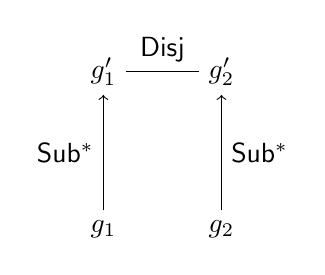
\begin{tikzpicture}
      \node (g1)  at (0,0) {$g_1$};
      \node (g2)  at (1.5,0) {$g_2$};
      \node (g1p) at (0,2) {$g_1'$};
      \node (g2p) at (1.5,2) {$g_2'$};
      \draw (g1p) to node[above] {$\mathsf{Disj}$} (g2p);
    %  \draw [->,decoration=snake,decorate]
     \draw [->,decoration=,decorate]
            (g1) to node[left] {$\mathsf{Sub^{*}}$} (g1p);
     % \draw [->,decoration=snake,decorate]
            \draw [->,decoration=,decorate]
            (g2) to node[right] {$\mathsf{Sub^{*}}$} (g2p);
    \end{tikzpicture}
   \end{center}
   \caption{Visualization of the protected pair $\setbr{g_1,g_2}$}\label{fig:protected}
   \end{figure}
  Thus, $S$ is protected if its two granules are (not necessarily
proper) subgranules of corresponding ones in a pair $S'$ which is
declared explicitly to be disjoint, either as a tautology or else as a
constraint of $\granschemaname{G}$.
 In this case, $S'$ is called a \emph{protector} of $S$.
   A pair $S \in \doubletsofgrsch{G}$ is \emph{unprotected (for
$\granschemaname{G}$)} if it is not protected.
    The set of all protected pairs for $\granschemaname{G}$ is denoted
  $\protectedprgrsch{G}$, while
  $\unprotectedprgrsch{G}
       = \doubletsofgrsch{G}  \setminus \protectedprgrsch{G}$
 is the set of unprotected pairs for $\granschemaname{G}$.
 \end{metalabpara}


 \begin{metaemphlabpara}{lemma}{Lemma}
         {Protection implies disjointness}\envlabel{lem:protected}
   For any $S \in \doubletsofgrsch{G}$,
 \nlrightt
  $S \in \protectedprgrsch{G}$ iff 
 $\pconstrgrsch{G} \sentails \disjrulesetp{S}$.
 \begin{proof}
     See \mycite[Thm.\ 3]{AtzeniPa88_dke}.
 \end{proof}
 \end{metaemphlabpara}


 \begin{metalabpara}{}{}
    {One- and two-path left-linear proofs
     for disjointness constraints}\envlabel{def:2pathlinear}
     Suppose that $\disjrulep{g_1}{g_2}$ is the constraint to prove.
There are four cases to consider.
     First of all, if $\disjrulep{g_1}{g_2} \in \pconstrgrsch{G}$,
then the constraint itself forms its proof tree.
     Second, if $\disjrulep{g_1}{g_2}$ is a tautology; that is, if
 $g_1 \ideq \botgrsch{G}$, then the proof tree is
 $\disjrulepbar{\botgrsch{G}}{g_2}{1.5}$
 (and analogously if $g_2 \ideq \botgrsch{G}$).
     Third, neither of these hold, but for some
  $g_1' \in \granulesofsch{G}$,
 $\disjrulep{g_1'}{g_2} \in \pconstrgrsch{G}$, then the proof is of
the form shown in Fig.\ \ref{fig:1pathlinear}.  An analogous result
holds $\disjrulep{g_1}{g_2'} \in \pconstrgrsch{G}$ for some
  $g_2' \in \granulesofsch{G}$.
   \begin{figure}[htb]
   \[
     \begin{prooftreem}
      \hypoi{\Sigma_1}
      \ellipsis{}{\mbox{left-linear proof}}
      \ellipsis{}{\subrulep{g_1}{g_1'}}
      \hypoi{\disjrulep{g_1'}{g_2}}
      \inferii{\disjrulep{g_1}{g_2}}
     \end{prooftreem}
   \]
   \caption{A one-path linear proof of disjointness}\label{fig:1pathlinear}
   \end{figure}
    Finally, if none of these holds, then the proof is as shown in
Fig.\ \ref{fig:2pathlinear}.
   \begin{figure}[htb]
   \[
     \begin{prooftreem}
      \hypoi{\Sigma_1}
      \ellipsis{}{\mbox{left-linear proof}}
      \ellipsis{}{\subrulep{g_1}{g_1'}}
      \hypoi{\Sigma_2}
      \ellipsis{}{\mbox{left-linear proof}}
      \ellipsis{}{\subrulep{g_2}{g_2'}}
      \hypoi{\disjrulep{g_1'}{g_2'}}
      \inferii{\disjrulep{g_1'}{g_2}}
      \inferii{\disjrulep{g_1}{g_2}}
     \end{prooftreem}
   \]
   \caption{A two-path linear proof of disjointness}\label{fig:2pathlinear}
   \end{figure}
 \end{metalabpara}


 \begin{metaemphlabpara}{proposition}{Proposition}
    {Deducing satisfiability of disjointness
                                  constraints}\envlabel{prop:infdisj}
     If
 \preformat{\linebreak}
 $\pconstrgrsch{G}$ is satisfiable, then for any
 $g_1, g_2 \in \granulesofsch{G}$ with
 $\pconstrgrsch{G} \sentails \disjrulep{g_1}{g_2}$,
 there is a single-use left-linear proof in $\bininfpos{G}$ of at most
two paths of this and using at most those rules which lie in
     $\setbr{\textup{(I2)},\textup{(M1)},\textup{(I1)},\textup{(T1)},
            \textup{(T2)},\textup{(T3)}}$.
 \begin{proof}
   The proof follows directly from the constructions of
\envref{def:2pathlinear}.  It only remains to show single usage.  In
all but the last case, it is trivial that the proof is single use.
For the last case, it suffice to note that since $g_1'$ and $g_2'$ are
disjoint, every granule in the path underlying $\grpr{g_1}{g_1'}$ must
be disjoint from every granule in the path underlying
$\grpr{g_2}{g_2'}$, so there is no possibility of a constraint being
used in both chains.
 \end{proof}
 \end{metaemphlabpara}


 \begin{metalabpara}{myexample}{Example}{}\envlabel{ex:pdeductsat}
   For a simple example of the proof technique of \envref{prop:infdisj},
   let
  $\granschemaname[\ref{ex:pdeductsat}]{G}$ be an SMAS with
 $\setdef{g_i}{i \in \ccinterval{1}{8}} \subseteq
           \granulesofsch[\ref{ex:pdeductsat}]{G}$
 and
   \newline
      $\setbr{\subrulep{g_1}{g_2}, \subrulep{g_2}{g_3}, \subrulep{g_3}{g_4},
             \subrulep{g_5}{g_6}, \subrulep{g_6}{g_7}, \subrulep{g_7}{g_8},
             \disjrulep{g_4}{g_8}}
    \nlrightt
       \subseteq
    \pbinconstrgrsch[\ref{ex:pdeductsat}]{G}$.
    \linebreak
   Assume further that $\pbinconstrgrsch[\ref{ex:pdeductsat}]{G}$ is
satisfiable.  In Fig.\ \ref{fig:pdeductsat} is shown a two-path
left-linear proof that
 $\pbinconstrgrsch[\ref{ex:pdeductsat}]{G}
           \sentails \disjrulep{g_1}{g_5}$
 using the proof rules of
 \preformat{\linebreak}
 $\bininfpos[\ref{ex:pdeductsat}]{G}$.
   \begin{figure}[htb]
   \[
     \begin{prooftreem}
      \hypoii{\subrulep{g_1}{g_2}}
             {\subrulep{g_2}{g_3}}
      \inferi{\subrulep{g_1}{g_3}}
      \hypoi{\subrulep{g_3}{g_4}}
      \inferii{\subrulep{g_1}{g_4}}
      \hypoii{\subrulep{g_5}{g_6}}
             {\subrulep{g_6}{g_7}}
      \inferi{\subrulep{g_5}{g_7}}
      \hypoi{\subrulep{g_7}{g_8}}
      \inferii{\subrulep{g_5}{g_8}}
      \hypoi{\disjrulep{g_4}{g_8}}
      \inferiii{\disjrulep{g_1}{g_5}}
     \end{prooftreem}
   \]
   \caption{Example proof of disjointness}\label{fig:pdeductsat}
   \end{figure}
 \end{metalabpara}


 \begin{metaemphlabpara}{proposition}{Proposition}
    {Deducing unsatisfiability
               using $\bininfpos{G}$}\envlabel{prop:bininfposfalse}
     If $\granschemaname{G}$ is not satisfiable, then there is a
single-use proof in $\bininfpos{G}$ whose last step is the application
of rule (U1).
  \begin{proof}
     The completeness of $\bininfpos{G}$ guarantees that there is a
proof of the unsatisfiability of $\granschemaname{G}$ whose last step
is an instantiation of (U1), since (U1) is the only rule which allows
the deduction of $\false$.  However, such an argument alone does not
guarantee the the proof will be single use.  To ensure that condition,
additional work is required.
    \par
    For the most general case, the idea of the proof is to build upon
previous results which ensure single-use proofs, specifically
\envref{prop:infdisj}.
    The strategy is to identify a granule
 $g \in \granulesofschnb{G}$ for which $\disjrulep{g}{g}$ is provable
from $\pconstrgrsch{G}$, in a form similar to that illustrated in
Fig.\ \ref{fig:2pathlinear}, and then append to the end of it an
application of (U1) to deduce $\false$, as illustrated in
Fig.\ \ref{fig:unsatproof}.
   \begin{figure}[htb]
   \[
     \begin{prooftreem}
      \hypoi{\Sigma_1}
      \ellipsis{}{\mbox{left-linear proof}}
      \ellipsis{}{\subrulep{g}{g_1'}}
      \hypoi{\Sigma_2}
      \ellipsis{}{\mbox{left-linear proof}}
      \ellipsis{}{\subrulep{g}{g_2'}}
      \hypoi{\disjrulep{g_1'}{g_2'}}
      \inferii{\disjrulep{g_1'}{g}}
      \inferii{\disjrulep{g}{g}}
      \inferi{\false}
     \end{prooftreem}
   \]
   \caption{A two-path linear proof of unsatisfiability}\label{fig:unsatproof}
   \end{figure}
    There are, however, two details which require attention.  First of
all, since $\pconstrgrsch{G}$ is unsatisfiable, care must be taken in
identifying what a proof is, since $\false$ entails anything and
everything.  Second, since $g$ is used in both linear paths, a
situation which does not occur in Fig.\ \ref{fig:2pathlinear}, it must
be ensured via other means that no rule is used more than once.
     \par
     The strategy is to switch to the proof system $\sqbininfpos{G}$
for all deductions of Fig.\ \ref{fig:unsatproof} except the last one
which deduces $\false$.  As established in \envref{prop:sqbininfpos},
any set of constraints is satisfiable in the context of strong
quasi-models.  Furthermore, every rule of $\bininfpos{G}$, save for
(U1), is also a rule of $\sqbininfpos{G}$.  Therefore, all of the tree
of Fig.\ \ref{fig:unsatproof} except the lowest level, in which (U1)
is applied, is also a proof tree in $\sqbininfpos{G}$.  Hence, the
entire tree is a proof tree in $\bininfpos{G}$.
     \par
    Now, let $p_1 = \abr{g_{11},g_{12},\ldots,g_{1k_1}}$
   (resp.\ $p_2 = \abr{g_{21},g_{22},\ldots,g_{2k_2}}$)
 be the path which underlies the proof of
  $\subrulep{g}{g_1'}$ from $\Sigma_1$
(resp.\ of $\subrulep{g}{g_2'}$ from resp.\ $\Sigma_2$).
 As in \envref{def:2pathlinear}, it is assumed that both $p_1$ and
$p_2$ are reduced.
   If $\Sigma_1 \intersect \Sigma_2 \neq \emptyset$, then some granule
other than $g$ must occur in both $p_1$ and $p_2$.  In that case, let
$g' \ideq g_{1i_1} \ideq g_{2i_2}$
 be the granule with the highest index in $p_1$ which also occurs in
 $p_2$, and replace
  $p_1$ with $p_1' = \abr{g_{1i_1},g_{1i_2},\ldots,g_{1k_1}}$,
  $p_2$ with $p_2' = \abr{g_{2i_1},g_{2i_2},\ldots,g_{2k_1}}$,
 and $g$ with $g'$ throughout the proof.
   The result is clearly single use, since for $\Sigma_1$ and
$\Sigma_2$ to have a constraint in common would require that $p_1$ and
$p_2$ have at least two granules in common.
     \par
   In the less general case, in which a final proof of false is
appended to a tree of the form of Fig.\ \ref{fig:1pathlinear}, the
proof similar but easier, since there is only one left-linear proof of
subsumption.  For the remaining possibilities (corresponding to the
first two cases of \envref{def:2pathlinear}), the proof is trivial.
  \end{proof}
 \end{metaemphlabpara}
   \parvert

    Finally, the main result of this section may be established.

 \begin{metaemphlabpara}{theorem}{Theorem}
    {$\bininfpos{G}$ and single use}\envlabel{thm:bininfpossingleuse}
    The proof system $\bininfpos{G}$ is sound, complete, and single
use.
 \begin{proof}
   This follows from \envref{prop:infsub}, \envref{prop:infdisj}, and
\envref{prop:bininfposfalse}.
 \end{proof}
 \end{metaemphlabpara}

 \begin{metalabpara}{myexample}{Example}{}\envlabel{ex:pdeductunsat}
   For a simple example of the proof technique of
\envref{prop:bininfposfalse}(b), let
  $\granschemaname[\ref{ex:pdeductunsat}]{G}$ be an SMAS with
 $\setdef{g_i}{i \in \ccinterval{1}{7}} \subseteq
           \granulesofsch[\ref{ex:pdeductunsat}]{G}$
 and
   \newline
      $\setbr{\subrulep{g_1}{g_2}, \subrulep{g_2}{g_3},
             \subrulep{g_3}{g_4},
             \subrulep{g_1}{g_5}, \subrulep{g_5}{g_6},
             \subrulep{g_6}{g_7},
             \disjrulep{g_4}{g_7}}
    \nlrightt
       \subseteq
    \pbinconstrgrsch[\ref{ex:pdeductunsat}]{G}$.
    \linebreak
   Assume further that
      $g_1 \not\ideq \botgrsch[\ref{ex:pdeductunsat}]{G}$.
   In Fig.\ \ref{fig:pdeductunsat} is shown a proof that 
 $\pbinconstrgrsch[\ref{ex:pdeductunsat}]{G}$ is unsatisfiable,
 using the proof rules of $\bininfpos[\ref{ex:pdeductunsat}]{G}$.
   \begin{figure}[htb]
    \[
     \begin{prooftreem}
      \hypoii{\subrulep{g_1}{g_2}}
             {\subrulep{g_2}{g_3}}
      \inferi{\subrulep{g_1}{g_3}}
      \hypoi{\subrulep{g_3}{g_4}}
      \inferii{\subrulep{g_1}{g_4}}
      \hypoii{\subrulep{g_1}{g_5}}
             {\subrulep{g_5}{g_6}}
      \inferi{\subrulep{g_1}{g_6}}
      \hypoi{\subrulep{g_6}{g_7}}
      \inferii{\subrulep{g_1}{g_7}}
      \hypoi{\disjrulep{g_4}{g_7}}
      \inferii{\disjrulep{g_1}{g_4}}
      \inferiisp{\disjrulesetp{\setbr{g_1}}}{separation=-1em}
      \inferi{\false}
     \end{prooftreem}
   \]
   \caption{Example proof of unsatisfiability}\label{fig:pdeductunsat}
   \end{figure}
 \end{metalabpara}





